\documentclass{standalone}

\usepackage{times}
\usepackage{amsmath}
\usepackage{amssymb}

\usepackage[dvipsnames]{xcolor}
\usepackage{tikz}
\usetikzlibrary{angles,arrows,backgrounds,scopes}

\usepackage{pgfplots}
\pgfplotsset{compat=1.15}
\begin{document}
	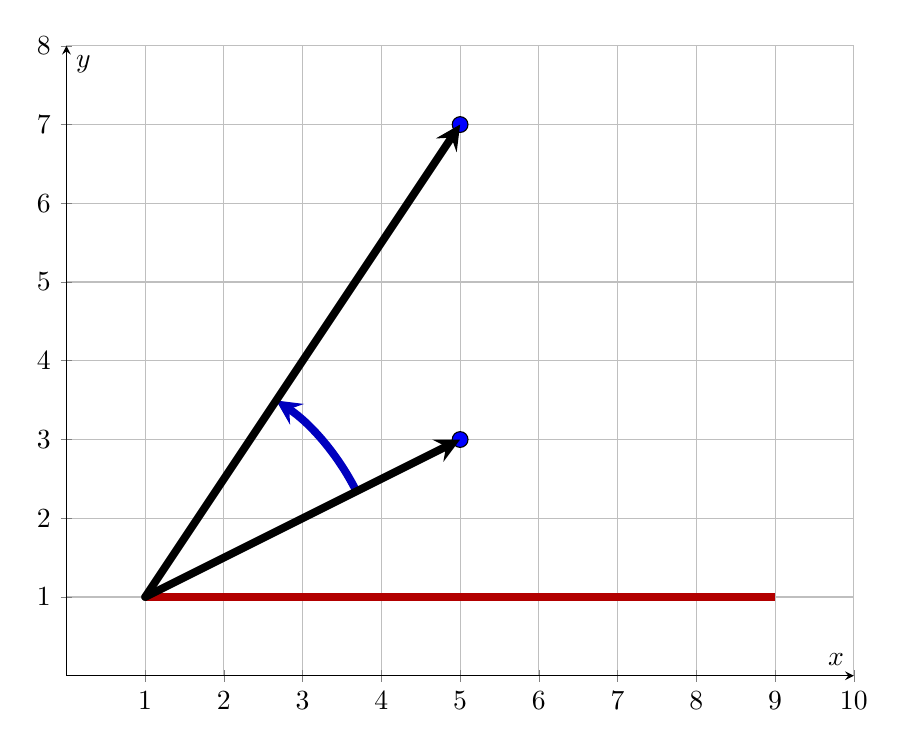
\begin{tikzpicture}[x=1cm,y=1cm]
		\begin{axis}[
			x=1cm,y=1cm,
			axis lines=middle,
			ymajorgrids=true,
			xmajorgrids=true,
			xmin=0,
			xmax=10,
			ymin=0,
			ymax=8,
			xtick={0,1,...,10},
			ytick={0,1,...,8},
			xlabel={$x$},
			ylabel={$y$},]
			\newcounter{visitorID}
			\draw[color=red!70!black,line width=0.1cm] (1,1)--(9,1);
		\end{axis}
		\newcommand{\visitor}[2]{
			\stepcounter{visitorID}
			%\node[fill=white,text opacity=1,fill opacity=0.66,inner sep=3pt,rounded corners=5pt] at (#1+0.2,#2-0.2) {$\arabic{visitorID}$};
			\draw [fill=blue] (#1,#2) circle (0.1);
			\coordinate (v\arabic{visitorID}) at (#1,#2);
		}
		%testdata:
		\visitor{5}{3}
		\visitor{5}{7}
		\coordinate (l) at (1,1);
		\coordinate (r) at (9,1);
		\pic [draw,blue!75!black, -stealth, angle radius=3cm,line width=0.1cm] {angle = v1--l--v2};
		\draw[-stealth,line width=0.1cm,line cap=round] (l)--(v1);
		\draw[-stealth,line width=0.1cm,line cap=round] (l)--(v2);
		
		%\pic [draw,blue!75!black, -stealth, angle radius=3cm,line width=0.1cm] {angle = v2--r--v1};
		%\draw[-stealth,line width=0.1cm,line cap=round] (r)--(v1);
		%\draw[-stealth,line width=0.1cm,line cap=round] (r)--(v2);
	\end{tikzpicture}
\end{document} 
